\documentclass{article}
\usepackage{times}
\usepackage{graphicx} % more modern
\usepackage{subfigure} 
\usepackage{natbib}
\usepackage{algorithm}
\usepackage{algorithmic}
\usepackage{hyperref}
\usepackage{amssymb}
\usepackage{amsmath}

\newcommand{\theHalgorithm}{\arabic{algorithm}}
\usepackage[accepted]{icml2016}

\usepackage{comment}
\newcommand{\compresslist}{
  \setlength{\itemsep}{1pt}
  \setlength{\parskip}{0pt}
  \setlength{\parsep}{0pt}}

%\yrcite{} if named otherwise \cite
\begin{document} 
\icmltitlerunning{LSTM for Text Generation and Classification}
\twocolumn[
\icmltitle{LSTM for Text Generation and Classsification}
\icmlauthor{Frédéric Boileau}{frederic.boileau@umontreal.ca}
\icmlauthor{Jimmy Leroux}{jimmy.leroux@umontreal.ca}
\icmlauthor{Nicolas Laliberté}{nicolas.laliberte@umontreal.ca}
\vskip 0.3in
]

\begin{abstract} 
    
In the context of our project for the IFT6269-A2018 we have investigated the
different available models for the generation and classification of natural
text data.  While we were initially interested in fully probabilistic models
such as Hidden Markov Models (HMM), a quick review of the contemporary
literature on the topic of pattern recognition on sequences made it clear that
neural networks (NN) provided the better toolset. In the end we implemented two
Long Short-Term Memory networks, for generation and classification respectively
which we trained on subsequences of some corpora of prose fiction. Despite the
rather coarse nature of our implementation the generators were able to produce
legible and decently structured text which reflected the material used for
training; in the style of the writing for example. The classifier reported 
excellent metrics however there are several interesting questions as to
what overfitting consists of when classifying prose fiction. The most
obvious is the one of proper nouns, but others such as temporal markers
are more subtle. The solutions to be decided with some context of the
intent of the task, so as to be the answer to a well-defined question.


\end{abstract} 

\medskip
\section{Introduction}

Hidden Markov Models used to be the go-to probabilistic tool to reason about
sequential data; the Markov assumption however proves to often be unreasonably
strong. Adding links to form higher order chains is not a scalable solution as
the computationnal complexity grows exponentially in the order of the chain.
Recurrent Neural Networks (RNN) constitute a family of neural network
architectures specialized to process sequential data which can forfeit
Markovian assumptions while remaining tractable.  RNNs can track longer range
dependencies while staying tractable by leveraging the simple idea of sharing
parameters across the model \cite{deeplearning}.  Concretely this means adding
loops to the hidden units of the neural network.  RNNs have been successfully
used in diverse domains for generating sequences such as music and text
\cite{gravesGenerating}.  Despite the aforementionned features, naive RNNs
suffer from the fact that the influence of some input to the hidden layer
either decays or blows up exponentially in time, a phenomenon reffered to in
the literature as the \textit{vanishing gradient problem}.  The cost of
abandonning probabilistic models such as the HMM in favor of neural networks is
the loss of a fully probabilistic interpretation. There has recently been an
increased interest into finding reasonable probabilistic interpretaions to
RNNs, see for example \cite{inter}. On the other hand the very existence of
some monolithic notion of ``interpretability'' has been recently questionned,
see \cite{mythos} for a philosophically inclined take on the question.

\section{Neural Networks Archicture}
\subsection{RNN and the Vanishing Gradient}
\begin{center}
    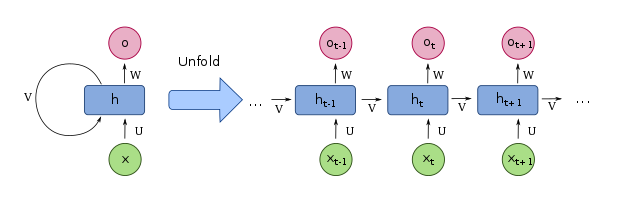
\includegraphics[width=\columnwidth]{RNN.png}
    \captionof{figure}{Unfolded RNN network. Figure taken from Christopher Olah's blog.}
\end{center}
\begin{equation*}
    h_t = \sigma(U x_t + V h_{(t-1)} + b_h)
    \quad o_t = \text{softmax}(W h_t + b_o)
\end{equation*}
Where $ U$, $V$ and $W$ are weights matrix and the vectors $b$ are bias
parameters. Consider the gradient of $o_{t + \delta}$ with respect
to $h_t$. Applying the chain rule according to the graph above we get:

\begin{equation*}
  \nabla_{h_t} o_{t + \delta} = \left( \prod_{k = t+1}^{t+\delta} V^T
  \text{diag}(h_k(1 - h_k)) \right)\nabla_{h_{t + \delta}}o_{t + \delta}.
\end{equation*}

Thus, as $\delta$ grows, the gradient grows exponentially with $V$. If $V$ is
small or large then the gradient will either vanish or explode. A myriad
of solutions exist such as regularization through weight noise, the Long Short
Term Memory architecture tries to tackle this issue on a higher level than
regularization.
\subsection{LSTM Architecture}
To go from a RNN to a LSTM we replace hidden units with components known as
\textit{memory cells}. Our presentation and notation follows \cite{revieww}.
\begin{center}
    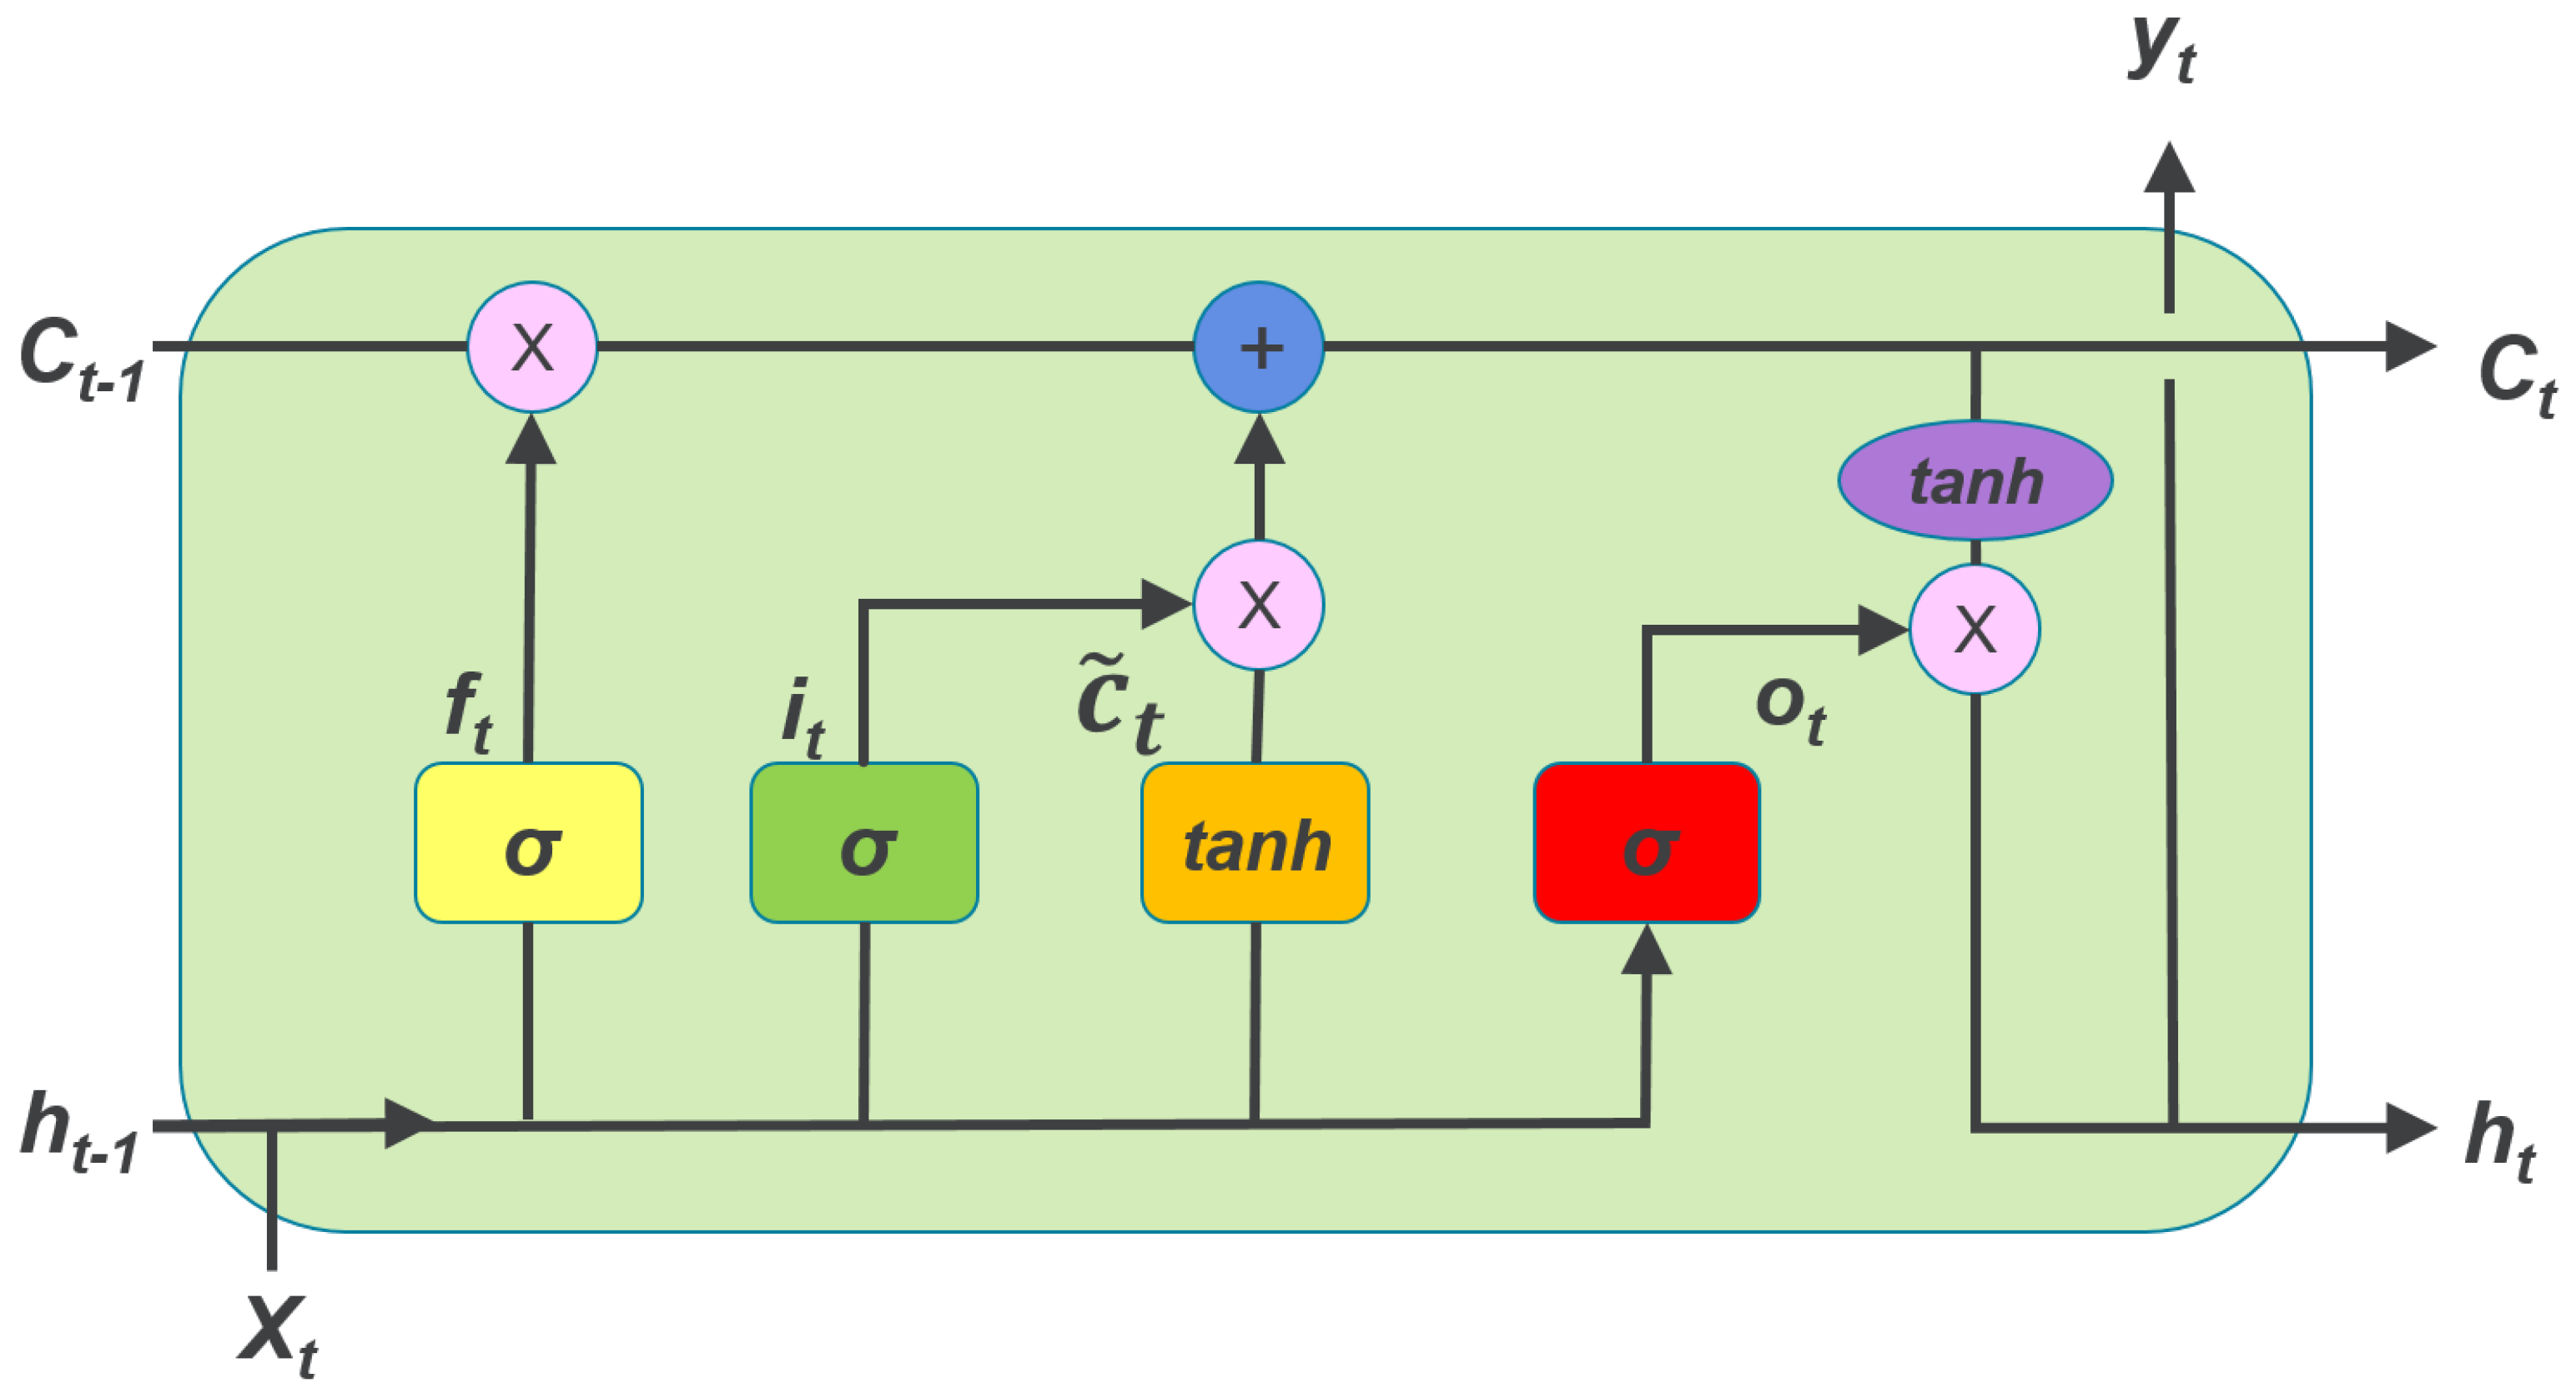
\includegraphics[width =\columnwidth]{lstm.png}
    \captionof{figure}{Memory cell of a LSTM. Figure taken from Christopher Olah's blog.}
\end{center}

Intuitively, RNNs have \textit{long-term memory} in the form of matrix weights,
they change during the training; encoding through training some general
knowledge about the data. They also have \textit{short-term memory} in the form
of activation passing from each node to successive ones. The memory cell
introduced in the LSTM model formalizes those notions and provides a framework
to control their impact on the internal representation of the network.
\begin{center}
    \begin{itemize}
    \item $f_t, i_t, o_t$: Respectively forget, input and output gates.
        \begin{itemize}
            \normalsize
            \item Sigmoidal units activated through  $x_t$ (current input) and
                $h_{t-1}$ (past hidden unit output) \item $f_t$ controls the
                recursive flow
            \item $i_t$ and $o_t$ control the input and output flow
                respectively
            \item $h_t = o_t \odot \tanh(c_t)$ where $\odot$ denotes element
                wise multiplication.
        \end{itemize}
    \item $c_t = \mathbf{f_t \odot c_{t-1}} + i_t \odot \tilde{c}_t$: The cell
    which has a self-connected edge with a fixed unit weight, thereby delegating
    control of recursion to the gate
    \end{itemize}
\end{center}
The architecture of the memory cell improves the capacity to learn long time 
dependencies. Indeed, following the definition of the cell state, we have
\begin{equation*}
	c_t = \sum_{k = o}^{t}f_t \odot \dots \odot f_{k + 1} \odot i_k \odot \tilde{c}_k.
\end{equation*}
We can see that the gradient may pass over long time gaps as long as the forget 
gates are open (closed to $1$) which can be achieved with a appropriate initialization
setting a large bias  for the gates $f$. 
 

\section{Implementation}
We now discuss training of the LSTM \textit{generators}. During initial
prototyping we trained on quite varied datasets to see how structure would
impact the generation. The four datasets were the Harry Potter novel series,
the Lord of The Rings series, a Kaggle dataset of jokes and a collection of
excerpts from shakespeare. This produced reasonable synthetic data (presented
below, note that the text for training is easily identifiable) and we
afterwards focused exclusively on prose fiction, selecting authors which seemed
\textit{close} in terms of style.  

The two text sequences of prose used for the subsequent training of generators
were two concatenated novels of Jane Austen and of George Eliot respectively.
All in English and utf-8 encoded.  Punctuation and structure was left
unprocessed.  Each dataset was split in sequences of 50 tokens (i.e.
``words'') and a dictionnary was built from the complete input ($\approx 60k$
unique tokens), defining the input space for the networks.  Vector encoding of
this space was used through an embedding layer mapping the words to a real
vector space of dimension 256.  Available embeddings such as \textit{word2vec}
and \textit{glove} were initally used but proved to be more cumbersome than our
own trained version. 

We trained four LSTM networks with the aforementionned data, a generator and a
classifier, once without preprocessing and another where the NLTK Part of
Speech Tagger (POS tagger) was used to filter out proper names and replace them
with generic ones from the \textit{names} dataset of the NLTK library. The
generic name replacement was shared across the Jane Austen and George Eliott
datasets. This was an effort to make the classifier be trained on rather
structural aspects of the prose, such as syntax, length of sentences and broad
notions of \textit{style} as opposed to simply directly matching vocabulary
which would have been trivial with the names of the characters.

Training was achieved at ``word'' level (tokenized with NLTK).
Character level had been previsously envisionned for the rest of the project as
it is more flexible and can \textit{learn new words and structural
information}\cite{gravesGenerating} for the generators). Despite this we kept
the training at word level for multiple reasons, the primary one being
robustness towards unicode characters which might vary between versions of the
text available and the second one being speed of convergence. 

To generate the sequences the trained generators were initialized with a random
word drawn from the dictionary and the most likely next word was fed back in
the network until the desired sequence length was reached. 1000 sequences (250
per model) were generated.  The classifier was trained on the original datasets
and were was then used to classify the generated synthetic data estimate which
dataset (or model, equivalently) was used for its generation, thereby giving us
some ``metric'' of the quality of the data.


\section{Empirical Results}

\subsection(Models details)

We used the many-to-one architecture like the one below for our 
classifier.
\begin{center}
	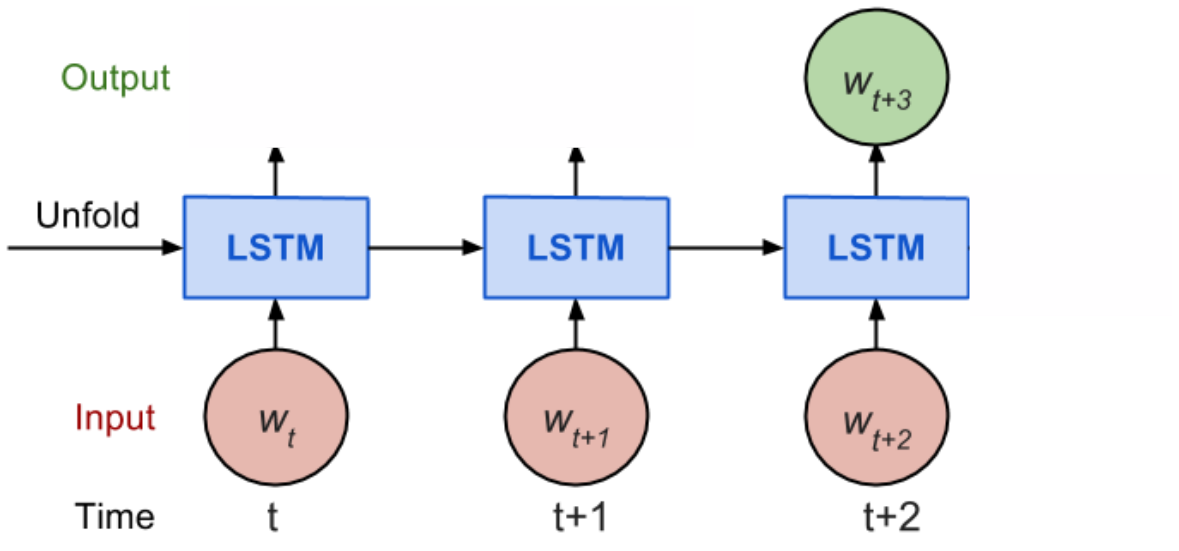
\includegraphics[width=.65\linewidth]{manytoone}
	\captionof{figure}{Many-to-one architecture.}
\end{center}
We used the last output of the LSTM as our input for the classifier, 
disregarding all the other outputs. The last hidden state contains 
information about about all the sequence through the memory cell. 

\begin{figure}[ht]
\vskip 0.2in
\begin{center}
\centerline{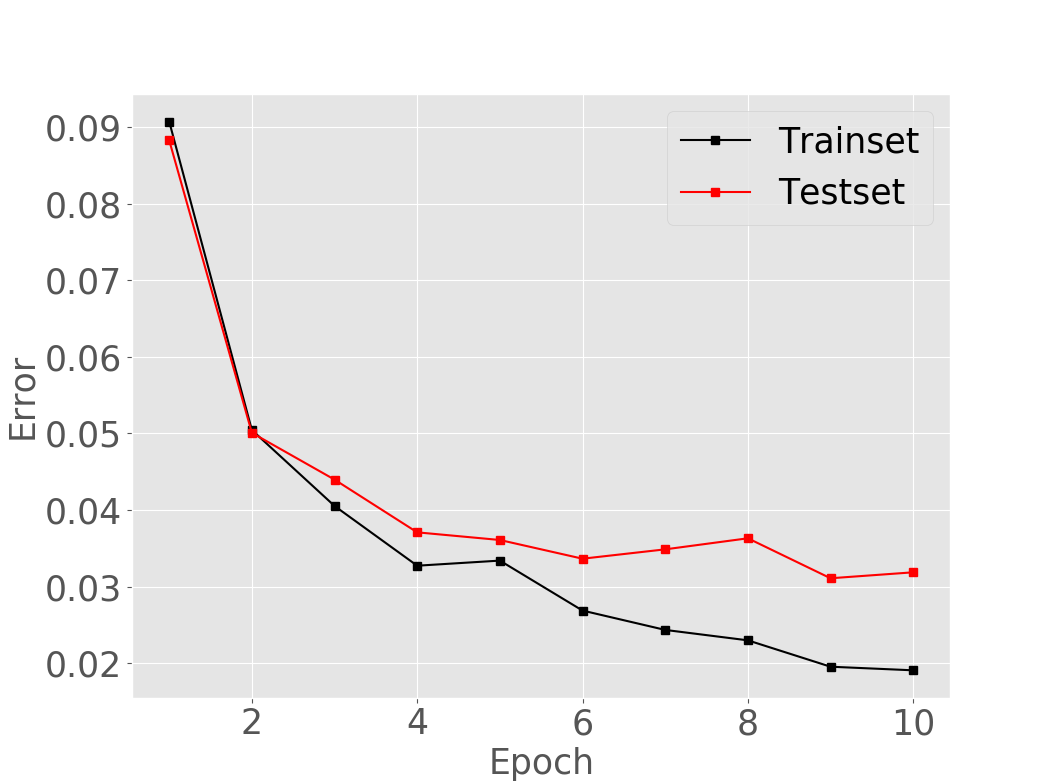
\includegraphics[width=\columnwidth]{classerror}}
\caption{Classification error on train/test set.}
\end{center}
\vskip -0.2in
\end{figure}

The error we used here is the cross-entropy loss, which is standard for 
classification tasks. We see on our training curves (figure 2) that we 
have reach 96\% for the classification accuracy.

\vspace{0.2in} 

For the text generation models, we used a many-to-many achitecture like 
the one showed in the RNN section with one layer for computational reasons.
LSTMs are with a cell state of 512 dimensions. We trained trough minimization 
of the cross-entropy loss, which is equivalent to\textit{perplexity}; the 
standard metric for language modeling \cite{gravesGenerating}.
\begin{figure}[htbp!]
\begin{tabular}{|l|l|c|}
\hline
Dataset & BPC & Perplexity \\
\hline
Harry Potter & 1.00 & 33 \\
LOTR & 1.02 & 35 \\
Random quotes & 1.10 & 45 \\
Shakespeare & 0.94 & 26\\
\hline
\end{tabular}
\end{figure}

Examples of generated quotes:
\begin{itemize}\compresslist
    \item `` well , we ' ll do it with a wand , '' said hermione . `` really ?
      '' said harry , looking at each other .
    \item  what looked about this
      way , the black citadel , was far from the
          darkness , the ring was heard , but the sea big was big , and a great
          ring was in his battle .
    \item failure is a beginning of love and a family which comes from god .
    \item  '' that now my mind shall screens his music , '' '' and i to give
      thee my vulgar heaven , '' '' i am your brother .
\end{itemize}

\section{Discussion}
\subsection{Stylometrics}
Authorship analysis is a field of computationnal linguistics where
the author's identity is to be extracted from the writing style of text.
\cite{stylo}. It has diverse applications beyond complementing the
work of traditionnal philologists such a fraud and plagiarism detection
or even identifying cybercriminals on underground forums\cite{doppel}.
Classically the field depended on statistical analysis 
of manually engineered features such as word frequency, length of 
sentences etc. 

Despite its great importance and the fact that it is fundamentally
quite well defined, i.e. the question who wrote this text
is more well posed than the ones concerning sentiment analysis for
example, there are major challenges. Clearly one needs to differentiate
between writing features specific to writing style as opposed to
context/ content specific features as Rosenthal and Yoon mention in 
their paper on the application of stylometric techniques to detect
multiple authorship in legal decision \yrcite{rosenthal}.

In this context the simple ``anonymization'' of the text sequences we performed
has the intent to disentangle the contextual features from the imprint of the
author. We have mentionned before that the classifier could be used as some
kind of metric on the synthetic data. Conversely, suppose one is fairly
confident in the quality of the generated text, i.e. after reading its content
and using some domain knowledge experts determines that it reflects quite well
the imprint of an author's style. In this case the generated data could be a
candidate for training of classifiers to detect authorship, when the data is
sparse for instance or simply because the very nature of synthetic data could
prevent overfitting to less relevant features, the author's footprint being in
some sense crystallized in the generator's features. Of course this is purely
circular if both directions are considered at the same time and we have found
the latter(using synthetic data to evaluate the generalization of the
classifier) to be more interesting both in the results it yields and in its
theoretical formulation.

In essence the goal would be to use text generation to trim from data all
contextual information that is not considered to be relevant in determining the
author (such as names or temporal and spatial markers in some cases) while
keeping the semantics of the text intact. Afterwards using that stripped text
to train the generators to obtain more synthetic data which reflects the author
in its structural semantics, beyond crude word frequency.  Of course the
question as to what to keep from the original text, what to trim and generally
what features constitute an author's footprint is one that for the moment
relies heavily on domain-knowledge, however, given that knowledge, LSTM can
leverage it to perform much deeper analyses than classical statistics provide,
relying on structure and not just isolated features.




\section{Conclusion and Further Work}
Through our project we have explored the different available methodologies for
the generation and classification of textual data. We explored both problems as
they seem complementary in some respects however for practical applications
classification is the most interesting and relevant. 

The most capable tools right now  for sequence classification and generation
revolve around NN and more precisely the LSTM architecture seems to be the go
to building block for those applications. One criticism of NN and deep learning
based pattern recognition techniques has revolved around notions of
\textit{interpretability}, however as Lipton discussed in his paper
\yrcite{inter} there is no single monolithic notion of interpretability. One of
the reasonable challenges he mentions is the one of \textit{contestability} of
the results of a model when we need ethical decision-making. Classical
stylometric techniques rely on statistics which are fairly easy to explain
and/or refute but the result from a LSTM might be harder to verify. This issue
can be adressed in many ways but first the notion that results need be
understandable by a reasonably educated person might seem over reaching as we
already rely on hard to contest forensic techniques such as DNA testing. To
adress this issue instead of simply dismissing it one might consider ways to
make the internal representation of a RNN model more cogent, ironically one
possible avenue Lipton suggests is to train a RNN to map the internal state of
the model used to a textual explanation.

One critical application of text classification is \textit{authorship analysis}
of which we have surveyed examples in diverse settings such as identifying
cyber criminals in underground forums or determining multiple authorship in
legal cases. 

We have obtained surprinsingly good results in both classification and text
generation despite our rather coarse training. The generative models clearly
learned some structural information, often matching speech marks in a
reasonable way, and yielding more complex sentence structures using hypotaxis
when trained from authors such as Jane Austen while using simpler shorter
sentences with conjunctives in the case of popular authors such as JK Rowling. 

In the case of classification for authorship analysis, overfitting seems to be
difficult to prevent without a clear methodology of what constitutes contextual
information and what is more intrisic to an author's style. As discussed before
there are many ways to answer this question and domain knowledge should not be
dismissed. Replacing character names in prose fiction by generic ones seems to
have reduced the confidence in our model. Explorations into what other
irrelevant features should be trimmed from the set is thus warranted such as
spatial markers. That is, obviously, when those markers are deemed irrelevant
to the task. In some cases, with larger datasets with many character names that
end up being shared across corpora, their choice by an author could very well
be considered to be relevant as markers of their style.


\section{Citations and References} 
\bibliography{example_paper}
\bibliographystyle{icml2016}
\end{document} 
